\documentclass[../main.tex]{subfiles}

\begin{document}
	\subsection{Low level features}


	The first step of computing features was to extract low level features and expose them so that I can engineer sophisticated features to train the classifiers on. In fact, For each building, I computed the facet adjacency graph --- \textit{c.f.} Figure~\ref{fig::geom_features} --- with meaningful information for each facet. I also computed the orthoprojection\footnote{Projection on the Plane $(O, \vec{\imath}, \vec{\jmath})$} of buildings and stored it in vectorial --- \textit{c.f.} Figure~\ref{fig::vector} --- and raster mode --- \textit{c.f.} Figure~\ref{fig::raster}.\\

	\thisfloatsetup{heightadjust=object}
	\begin{figure}[H]
		\ffigbox[\FBwidth]
		{
			\begin{subfloatrow}[2]
				\captionsetup{labelformat=brace, justification=raggedright}
				\ffigbox[\FBwidth]
				{\caption{Raster orthoprojection.}\label{fig::raster}}{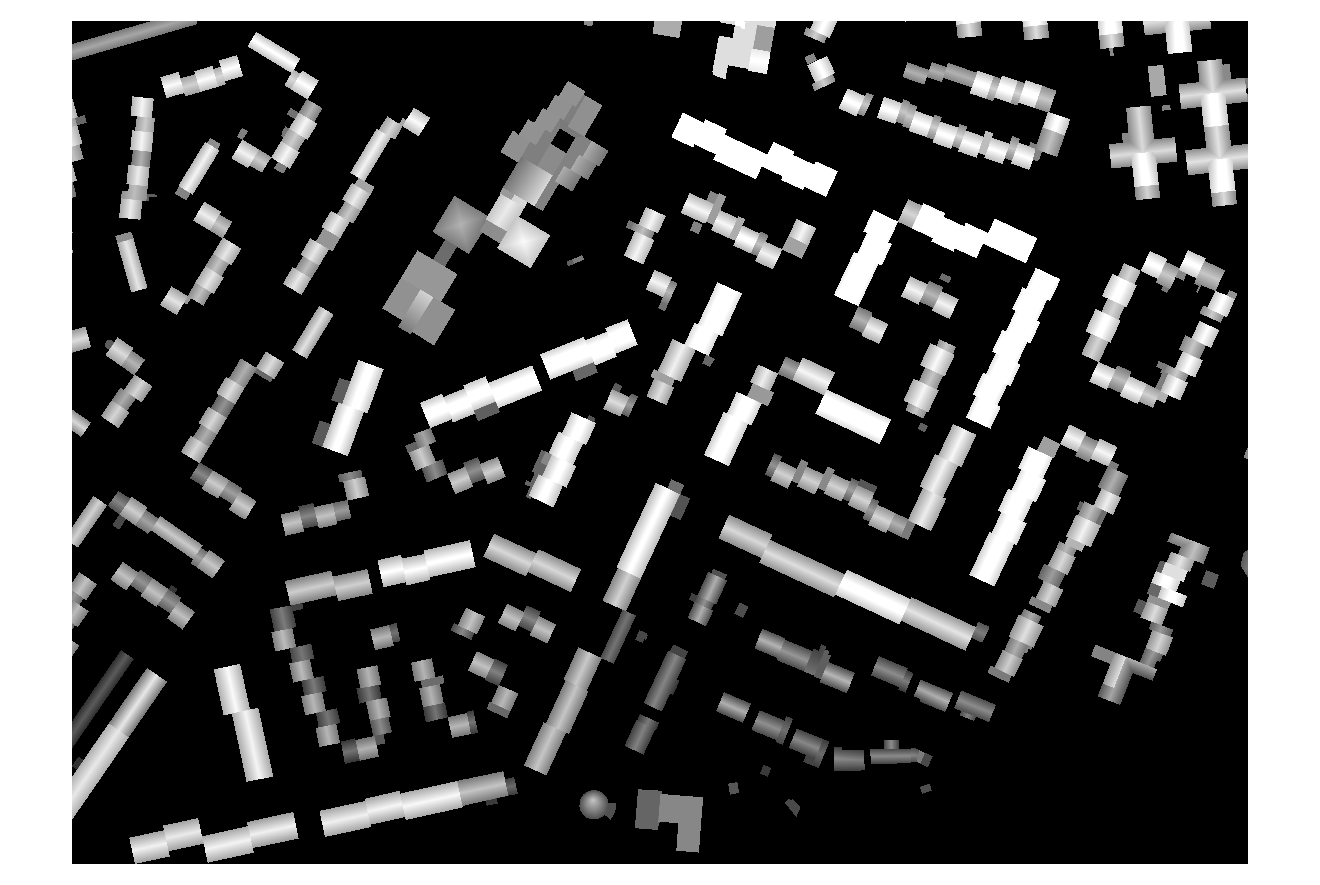
\includegraphics[width=.48\textwidth]{../images/raster/raster_projection}}
				\ffigbox[\FBwidth]{\caption{Vector orthoprojections (in transparent blue).}\label{fig::vector}}{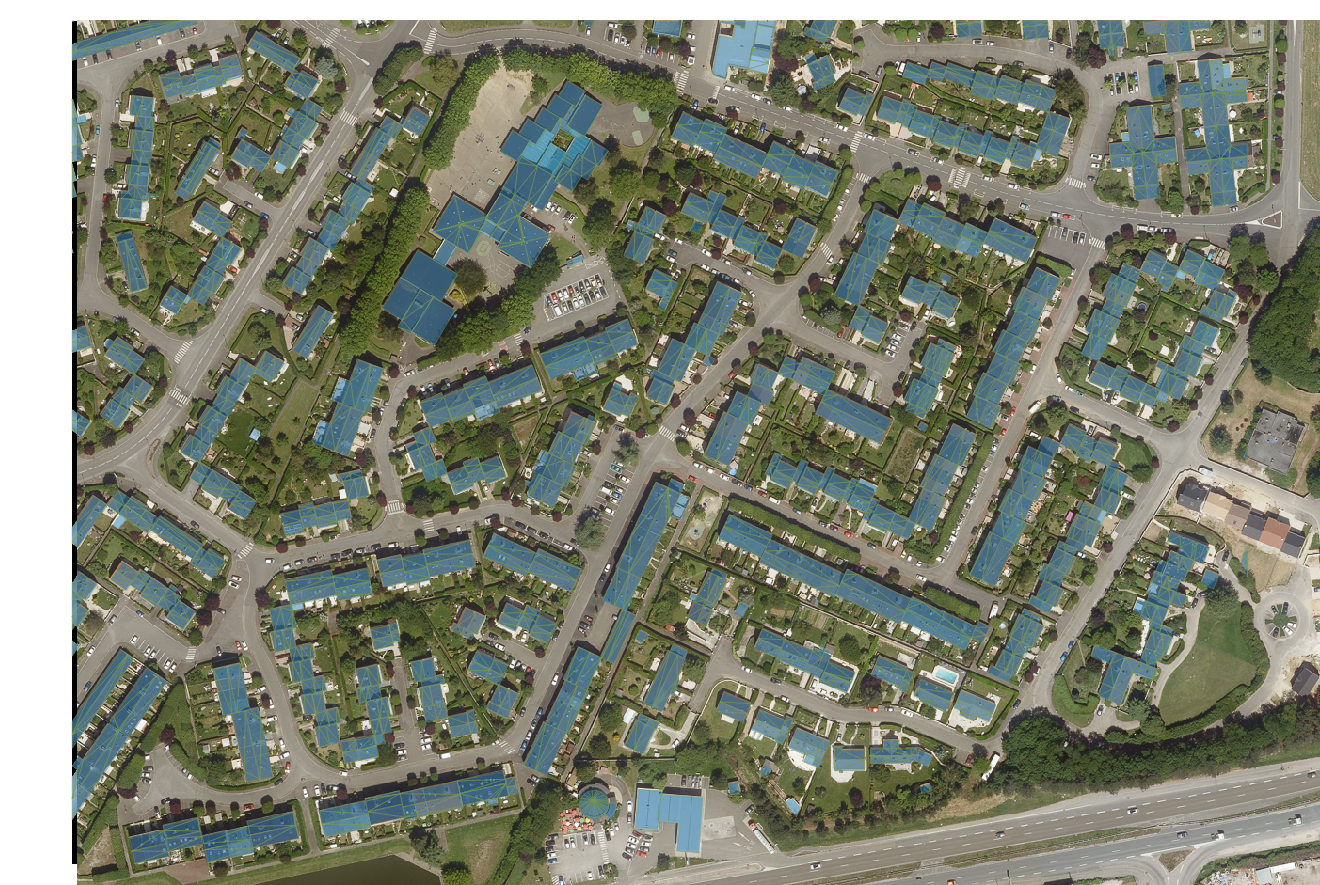
\includegraphics[width=.48\textwidth]{../images/raster/vector_projection}}
			\end{subfloatrow}
		}
		{
			\caption{\label{fig::orthoproj}Scene orthoprojections.}
		}
	\end{figure}

	\begin{figure}[H]
		\includestandalone[mode=buildnew, scale=1]{dual_features}
		\caption{\label{fig::geom_features} Low level geometric features per building.}
	\end{figure}
	\clearpage

	\subsection{Mid level features}
~\\

	The previous features are raw and not useful for classification. As a first
	step, in order to establish a baseline for the qualification, I choose simple
	features that can be classed as follows:
	\begin{itemize}
		\item[(i).] Geometric --- or intrinsic --- features: based on the graph adjacency features and the vector orthoprojections, I tried the feature vector per building in equation~\ref{eq::feature_vec}:
		\begin{equation}\label{eq::feature_vec}
			\text{feature\_vector} = \begin{bmatrix}
				statistics(degree_{facets})\\
				statistics(areas_{facets})\\
				statistics(centroid_{facets})\\
				statistics(normals_{facets})\\
				statistics(nomals\_with\_relations_{facets})
		\end{bmatrix}
		\end{equation}
		where:
		\begin{equation}
			statistics: property \mapsto \begin{bmatrix}
			\max_{facets}(property)\\
			\min_{facets}(property)\\
			mean_{facets}(property)\\
			median_{facets}(property)
		\end{bmatrix}
		\end{equation}
		\item[(ii).] Altimetric features: using the raster projections and the provided DSM, I computed the difference and used the its histogram as a feature vector. I can also try Bredif's method for DSM roof fitting later on.
		\item[(iii.)] Image features: left for later.
	\end{itemize}

	For now, I have focused on geometric features and altimetic features to complete the whole classification pipeline.The graph kernel methods and ortho image features are left for later. I should also grow my labelled datasets and invistigate other regions by active learning: transforming the pipeline to an active setting.
\end{document}
